% enable this to activate the version for PRINT
% disable this to make the pdf symmetric and without white pages
% => asymmetric alternating left/right margins
% \newcommand*{\printversion}{}%

%% | ---------------- document meta information --------------- |

\newcommand{\Author}{Ing. John Smith}
\newcommand{\Department}{Department of Cybernetics}
\newcommand{\Supervisor}{Ing. My Supervisor, Ph.D.}
\newcommand{\SupervisorSpecialist}{Ing. My Specialist, Ph.D.}
\newcommand{\Programme}{Insert My Study Programme Name}
\newcommand{\Field}{Insert My Study Subprogramme Name}
\newcommand{\Title}{My Thesis Title\\[0.5em]can Span Multiple Lines}
\newcommand{\DocName}{Doctoral Thesis}
\newcommand{\Keywords}{Unmanned Aerial Vehicles, Automatic Control}
\newcommand{\KlicovaSlova}{Bezpilotní Prostředky, Automatické Řízení}
\newcommand{\Year}{2021}
\newcommand{\Month}{January}
\newcommand{\Date}{\Month~\Year}
\newcommand{\Location}{Prague}

%% | ---------------------- configuration --------------------- |

% most of the configuration stuff happens here
%!TEX root = ../main.tex

%% | ----------------------- page setup ----------------------- |

% define documentclass based on the print/screen version of the document
\pdfoutput=1
\ifdefined\printversion
  \documentclass[a4paper,11pt,twoside,openright]{book}
\else
  \documentclass[a4paper,11pt,oneside]{book}
\fi

% define how "clearpage" works with the print/screen version of the document
\newcommand{\conditionalClearPage}{
  \ifdefined\printversion
    \cleardoublepage
  \else
    \clearpage
  \fi
}

%% | ----------------- commonly used packages ----------------- |

\usepackage[english]{babel}
\usepackage[utf8]{inputenc}
\usepackage{csquotes}
\usepackage{amsmath,amsfonts,amssymb,bm}
\usepackage{nicefrac}
\usepackage{algorithm,algpseudocode}
\usepackage[title,titletoc]{appendix}
\usepackage{latexsym}
\usepackage{a4wide}
\usepackage{color}
\usepackage{indentfirst}
\usepackage{graphicx}
\usepackage{fancyhdr,lastpage}
\usepackage{longtable}
\usepackage{pifont}
\usepackage{makeidx}
\usepackage{multirow}
\usepackage{dcolumn}
\usepackage{epstopdf}
\usepackage{url}
\usepackage{listings}
\usepackage{relsize}
\usepackage{pdfpages}
\usepackage{url}
\usepackage{lipsum}
\usepackage{isotope}
\usepackage{verbatim}
\usepackage{xcolor}
\usepackage{tcolorbox}
\usepackage[hidelinks]{hyperref}
\usepackage{multicol}
\usepackage{subfig}
\usepackage[export]{adjustbox}

% print version has different margins to accommodate the spine of the book
% do not move this around, or it stops working
\ifdefined\printversion
  \usepackage[a4paper,margin=3.2cm,inner=3.4cm,outer=2.0cm]{geometry}
\else
  \usepackage[a4paper,margin=3.2cm,inner=2.7cm,outer=2.7cm]{geometry}
\fi

\hyphenation{}

%% | ---------------------- abbreviations --------------------- |

\usepackage[printonlyused]{acronym}

% use to change margins around abbreviations block
\def\changemargin#1#2{\list{}{\rightmargin#2\leftmargin#1}\item[]}
\let\endchangemargin=\endlist

%% | -------------------------- tikz -------------------------- |

\usepackage{tikz}
\usepackage{pgfplots}
\pgfplotsset{compat=1.14}
\usetikzlibrary{backgrounds,arrows,automata,shapes,positioning,calc,through,spy,shapes,shapes.geometric,shapes.multipart,fit,patterns,fadings}
\pgfdeclarelayer{background}
\pgfdeclarelayer{foreground}
\pgfsetlayers{background,main,foreground}

%% | ------------ siunitx for units of measurements ----------- |

\usepackage{siunitx}
\DeclareSIUnit \parsec {pc}
\DeclareSIUnit \electronvolt {eV}
\DeclareSIUnit \pixel {px}
\DeclareSIUnit \arcmin {arcmin}
\DeclareSIUnit \erg {erg}
\DeclareSIUnit \joul {J}

%% | --------------- change formatting of lists --------------- |

\usepackage{enumitem}
\setlist{nosep}

%% | -------------------- table of contents ------------------- |

\usepackage[subfigure]{tocloft}

\tocloftpagestyle{plain}

%% | ----------------- formatting of a chapter ---------------- |

\usepackage{titlesec}
\titleformat{\chapter}[block]
{\normalfont\huge\bfseries}{Chapter \thechapter\\\vspace{0.1em}\\}{1em}{\Huge}
% {?}{before}{after}
\titlespacing*{\chapter}{0pt}{-1em}{2em}

%% | ------------------------ biblatex ------------------------ |

\usepackage[backend=bibtex,defernumbers=true,style=ieee,sorting=ydnt,sortcites=true]{biblatex}

% define the source file with bibliography
\addbibresource{main.bib}

\renewcommand*{\bibfont}{\Font}

% add suffix "a" to publications containing the keyword "mine"
% add suffix "c" to publications containing the keyword "mine" && "core"
\DeclareFieldFormat{labelnumber}{%
  \ifkeyword{mine}
    {\ifkeyword{core}
      {{\number\numexpr#1}c}%
      {{\number\numexpr#1}a}%
    }%
    {#1}%
}

\DeclareCiteCommand{\tabcite}%[\mkbibbrackets]
  {\usebibmacro{cite:init}%
   \usebibmacro{prenote}}
  {\usebibmacro{citeindex}%
   \usebibmacro{cite:comp}}
  {}
  {\usebibmacro{cite:dump}%
   \usebibmacro{postnote}}

% define fullciteinbox command
\definecolor{light-gray}{gray}{0.95}
\newcommand{\fullciteinbox}[2]{%

\DeclareCiteCommand{\fullcite}
{\usebibmacro{prenote}}
{\clearfield{addendum}%
  \usedriver
  {\defcounter{minnames}{6}%
  \defcounter{maxnames}{6}}
{\thefield{entrytype}}}
{\multicitedelim}
{\usebibmacro{postnote}}

\begin{tcolorbox}[width=\textwidth,colback={light-gray},title={}]%
\ifx&#2&
\else
  \textbf{#2}:\\\\
\fi
\begin{minipage}[t]{0.07\linewidth}%
\raggedright%
\cite{#1}%
\end{minipage}%
\begin{minipage}[t]{0.93\linewidth}%
\fullcite{#1}%
\end{minipage}%
\end{tcolorbox}%
%}%
\vspace{-0.3em}
}%

% change the bibliography font style
% does not compile without this
\let\bibfont\small

%% | ---------------------- custom macros --------------------- |

\newcommand{\strong}[1]{\textbf{#1}}
\newcommand{\coord}[1]{\textbf{#1}}
\newcommand{\norm}[1]{\left\lvert#1\right\rvert}
\newcommand{\m}[1]{\ensuremath{\mathbf{#1}}}
\newcommand\numberthis{\addtocounter{equation}{1}\tag{\theequation}}
\newcommand{\add}[1]{{\color{green} {#1}}}
\newcommand{\todo}[1]{{\color{red} TODO {#1}}}
\newcommand{\updated}[1]{{\color{blue} {#1}}}
\newcommand{\real}{\mathbb{R}}
\newcommand{\red}[1]{{\color{red} #1}}
\newcommand{\minus}{\scalebox{0.75}[1.0]{$-$}}
\newcommand{\plus}{\scalebox{0.8}[0.8]{$+$}}
\newcommand{\figvspace}{\vspace{-1em}}

% referencing
\newcommand{\reffig}[1]{Fig.~\ref{#1}}
\newcommand{\refalg}[1]{Alg.~\ref{#1}}
\newcommand{\refsec}[1]{Sec.~\ref{#1}}
\newcommand{\reftab}[1]{Table~\ref{#1}}
\newcommand{\refeq}[1]{\eqref{#1}}

%% | --------------- change listings and itemize -------------- |

\lstset{breaklines=true,captionpos=b,frame=single,language=sh,float=h}
\lstloadlanguages{sh,c}
\def\lstlistingname{Listing}
\def\lstlistlistingname{Listings}

%% | -------------------- layout parameters ------------------- |

% no indent, free space between paragraphs
\setlength{\parindent}{1cm}
\setlength{\parskip}{1ex plus 0.5ex minus 0.2ex}

% offsets the head down
\setlength{\headheight}{18pt}

% foot line
\renewcommand{\footrulewidth}{0.4pt}

%% | -------------- define the 'full' page style -------------- |

\fancypagestyle{full}{%

  % clear the default layout
  \fancyhead{}
  \fancyfoot{}

  % page header
  \fancyhead[LO]{\leftmark}
  \fancyhead[RE]{\rightmark}
  \fancyhead[LE,RO]{\thepage/\pageref{LastPage}}

  % page footer
  \fancyfoot[L]{CTU in Prague}
  \fancyfoot[R]{\Department}
  \fancyfoot[C]{}
}

%% | -------------- define the 'plain' page style ------------- |

\fancypagestyle{plain}{%

  % clear the default layout
  \fancyhead{}
  \fancyfoot{}

  % page header
  \fancyhead[LE,RO]{\thepage}
}

%% | -------------- Adjust style of chapter names ------------- |

\renewcommand{\chaptermark}[1]{\markboth{\MakeUppercase{\thechapter.\ #1}}{}}

%% | -------- European layout, no extra space after '.' ------- |

\frenchspacing

%% | ----------- adjust the style of the first page ----------- |

\makeatletter
\renewcommand\chapter{\if@openright\cleardoublepage\else\clearpage\fi
                    \thispagestyle{full}% original style: plain
                    \global\@topnum\z@
                    \@afterindentfalse
                    \secdef\@chapter\@schapter}
\makeatother


%% | ---------------------- the contents ---------------------- |

\begin{document}

%% --------------------------------------------------------------
%% |                         Title page                         |
%% --------------------------------------------------------------

\begin{titlepage}
  \begin{center}

    \textsc{\Large Czech Technical University in Prague}\\[1em]
    \textsc{\large Faculty of Electrical Engineering\\
    Department of Cybernetics\\
    Multi-robot Systems\\[3em]
    }
    
\includegraphics[height=4.1cm]{fig/ctu_lion.pdf}\\[3em]

    \textbf{\textsc{\Huge \Title}}\\[2em]

    \textbf{\Large \DocName}\\[6em]

    \textbf{\huge \Author}\\[6em]

    {\large \Location, \Date}\\[3em]

    Study programme: \Programme\\
    Branch of study: \Field\\[2em]

    \textbf{Supervisor: \Supervisor}\\
    \textbf{Supervisor-Specialist: \SupervisorSpecialist}

    \vspace{2pt}

  \end{center}
\end{titlepage}


% set up the page style for the "intro" pages
\pagestyle{plain}
\conditionalClearPage
\pagenumbering{roman}

%% --------------------------------------------------------------
%% |                       Acknowledgments                      |
%% --------------------------------------------------------------

../../common_resources/src/acknowledgments.tex

%% --------------------------------------------------------------
%% |                          Copyright                         |
%% --------------------------------------------------------------

\conditionalClearPage
%!TEX root = ../main.tex

\begin{changemargin}{0.8cm}{0.8cm}

~\vfill{}

\section*{Copyright}
\vskip 0.5em

This thesis is a compilation of several articles published and submitted during my Ph.D. studies.
The included publications are presented under the copyrights of IEEE, and Springer for posting the works for internal institutional uses.
The works are protected by the copyrights of respective publishers and can not be further reprinted without the publishers' permission.

\vskip 1.0cm

\textsuperscript{\textcopyright} IEEE, 2020\\
\textsuperscript{\textcopyright} Springer, 2020\\

\end{changemargin}


%% --------------------------------------------------------------
%% |                          Abstracts                         |
%% --------------------------------------------------------------

\conditionalClearPage
../../common_resources/src/abstract_en.tex

\conditionalClearPage
../../common_resources/src/abstrakt_cz.tex

\conditionalClearPage

%% --------------------------------------------------------------
%% |                        Abbreviations                       |
%% --------------------------------------------------------------

\begin{changemargin}{0.8cm}{0.8cm}

~\vfill{}

\section*{Abbreviations}

% this will print only the used abbreviations
%!TEX root = ../main.tex

\begin{acronym}
  \acro{API}[API]{Application Programming Interface}
  \acro{CTU}[CTU]{Czech Technical University}
  \acro{DOF}[DOF]{degree-of-freedom}
  \acro{FOV}[FOV]{Field of View}
  \acro{GNSS}[GNSS]{Global Navigation Satellite System}
  \acro{GPS}[GPS]{Global Positioning System}
  \acro{IMU}[IMU]{Inertial Measurement Unit}
  \acro{LKF}[LKF]{Linear Kalman Filter}
  \acro{LTI}[LTI]{Linear time-invariant}
  \acro{LiDAR}[LiDAR]{Light Detection and Ranging}
  \acro{MAV}[MAV]{Micro Aerial Vehicle}
  \acro{MPC}[MPC]{Model Predictive Control}
  \acro{MRS}[MRS]{Multi-robot Systems Group}
  \acro{ROS}[ROS]{Robot Operating System}
  \acro{RTK}[RTK]{Real-time Kinematics}
  \acro{SLAM}[SLAM]{Simultaneous Localization And Mapping}
  \acro{UAV}[UAV]{Unmanned Aerial Vehicle}
  \acro{UGV}[UGV]{Unmanned Ground Vehicle}
  \acro{UKF}[UKF]{Unscented Kalman Filter}
\end{acronym}


\vskip 2.5cm

\end{changemargin}

\conditionalClearPage

%% --------------------------------------------------------------
%% |                      Table of contents                     |
%% --------------------------------------------------------------

\tableofcontents

\conditionalClearPage

% set up the full page style
\pagestyle{full}

%% --------------------------------------------------------------
%% |                        introduction                        |
%% --------------------------------------------------------------

\chapter{Introduction}

\pagenumbering{arabic}

First, introduce the reader to the research topic.
Start with the most general view and slowly converge to the particular field, subfield, and the challenges you face.
You can cite others work here \cite{baca2020mrs}.

\section{Related works}

This section should contain related state-of-the-art works and their relation to the author's work.
We usually cite the original works like this \cite{benallegue2008high}.
You can also cite multiple papers at once like this \cite{baca2016embedded, baca2020mrs}.

\section{Contributions}

This section should briefly describe the author's contributions to his field of research.


%% --------------------------------------------------------------
%% |                How to write thesis in LaTeX                |
%% --------------------------------------------------------------

%!TEX root = ../main.tex

\chapter{How to write thesis in LaTeX\label{chap:how_to}}

\section{Versioning with git}

Write the LaTeX in such a way that it could be versioned by git, which will help when collaborating with other people.
This means writing \textbf{one sentence per line}.
Even when you use third-party platforms, such as the OverLeaf, you can still share the repository through Git.

\section{Mathematical notation with LaTeX}

Use bold to visually distinguish vectors and matrices ($\mathbf{x}$, $\mathbf{A}$) and scalars ($k$, $N$).
Mathematical equations should be numbered and should be part of a sentence.
For example, the following equation is a discrete LTI system update
\begin{equation}
  \mathbf{x}_{\left[k+1\right]} = \mathbf{A}\mathbf{x}_k + \mathbf{B}\mathbf{u}_k,
  \label{eq:lti_system}
\end{equation}
where $\mathbf{x}_k \in \mathbb{R}^m$ is the state vector at the sample $k$, $\mathbf{u}_k \in \mathbb{R}^n$ is the input vector, $\mathbf{A} \in \mathbb{R}^{m \times m}$ is the main system matrix, and $\mathbf{B} \in \mathbb{R}^{m \times n}$ is the system input matrix.
Proper punctuation should be used after \refeq{eq:lti_system}, as if it were an ordinary object in the sentence.
Do not put any empty lines around the equation.
That would create a new paragraph mid-sentence.

\section{Using footnotes}

Do not be afraid to use footnotes for additional information, such as http links\footnote{This repository: \url{https://github.com/ctu-mrs/thesis_template}.}.
We use footnote links whenever we want to \emph{point} to a website, rather then to cite it as a source.
Like with everything, do not overdo it.

\section{Referencing to document elements}

LaTeX allows you to dynamically reference to parts of the documents, such as
\begin{itemize}
  \item figures: \reffig{fig:uavs}, Figure\,\ref{fig:uavs},
  \item equations: \refeq{eq:lti_system},
  \item code: \reflst{lst:references},
  \item and any other object that can contain \texttt{label}.
\end{itemize}

Check the section in the \texttt{document\_setup.tex} that contains useful macros for unifying the references:

\begin{lstlisting}[caption={LaTeX macros for referencing to document elements.},label={lst:references}]
  \newcommand{\reffig}[1]{Fig.~\ref{#1}}
  \newcommand{\reflst}[1]{Lst.~\ref{#1}}
  \newcommand{\refalg}[1]{Alg.~\ref{#1}}
  \newcommand{\refsec}[1]{Sec.~\ref{#1}}
  \newcommand{\reftab}[1]{Table~\ref{#1}}
  \newcommand{\refeq}[1]{\eqref{#1}}
\end{lstlisting}

\section{Abbreviations with Acronym}

Abbreviations are handled by the \emph{acronym} package.
Example sentence with abbreviations: ``\ac{UAV} is a flying vehicle that commonly uses \ac{LiDAR} and \ac{GPS} receiver''.
Please, read the documentation\footnote{Acronym package: \url{http://mirrors.ctan.org/macros/latex/contrib/acronym/acronym.pdf}}.

\section{Units of measurements with Siunitx}

Typesetting of units has never been more accessible with the Siunitx package.
Acceleration is measure in \si{\meter\per\second\squared}.
Gravity accelerates objects at a rate $\approx \SI{9.81}{\meter\per\second\squared}$ near the sea level.
You can define your units if you want.

\section{2D Diagrams with Tikz}

\emph{Tikz} is a powerful tool for drawing 2D (and 3D) shapes and diagrams.
Check the documentation and examples: \url{https://www.overleaf.com/learn/latex/TikZ_package}.
The benefit of using \emph{Tikz}, instead of some other third-party drawing program, are:
\begin{itemize}
  \item fonts are the same as in LaTeX,
  \item you can typeset math in LaTeX,
  \item you can use references to other parts of your document,
  \item you can version the image in git,
  \item the images are easily adjustable while editing your document.
\end{itemize}
Check \reffig{fig:pgfplots} for example.

\begin{figure}[!h]
  \centering

  \begin{adjustbox}{max totalsize={0.6\textwidth}{0.90\textheight}, center}
    \tikzset{
  >=stealth',
  punkt/.style={
    rectangle,
    rounded corners,
    draw=black, very thick,
    text width=5.7em,
    minimum height=2em,
    text centered,
  },
  small_punkt/.style={
    rectangle,
    rounded corners,
    draw=black, very thick,
    text width=4.0em,
    text centered,
  },
  arrow/.style={
    ->,
    very thick,
    shorten <=2pt,
    shorten >=2pt,
  },
  arrow_red/.style={
    ->,
    draw=red, very thick,
    shorten <=2pt,
    shorten >=2pt,
  },
}

\begin{tikzpicture}[node distance=1cm, auto,]

  % outer circle nodes
  \node[punkt] (sensor) {Sensor size};
  \node[punkt, inner sep=5pt, below = of sensor, shift = {(-6.0, -0.75)}] (aircraft) {Aircraft\\size};
  \node[punkt, inner sep=5pt, below = of sensor, shift = {(0.0, -4.0)}] (constraints) {Environment constraints};
  \node[punkt, inner sep=5pt, below = of sensor, shift = {(6.0, -0.75)}] (strategy) {Localization strategy};

  % inner circle nodes
  \node[small_punkt, inner sep=5pt, below = of sensor, shift = {(0.0, 0.5)}] (sensor2) {\scriptsize Sensor size};
  \node[small_punkt, inner sep=5pt, right = of aircraft, shift = {(0.5, -0.0)}] (aircraft2) {\scriptsize Aircraft\\size};
  \node[small_punkt, inner sep=5pt, above = of constraints, shift = {(0.0, -0.5)}] (constraints2) {\scriptsize Environment\\constraints};
  \node[small_punkt, inner sep=5pt, left = of strategy, shift = {(-0.5, -0.0)}] (strategy2) {\scriptsize Localization\\strategy};

  \path[->] ($(sensor.west)+(0, 0)$) edge [arrow,bend right=45] ($(aircraft.north)$);
  \path[->] ($(aircraft.south)+(0, 0)$) edge [arrow,bend right=45] ($(constraints.west)$);
  \path[->] ($(constraints.east)+(0, 0)$) edge [arrow,bend right=45] ($(strategy.south)$);
  \path[->] ($(strategy.north)+(0, 0)$) edge [arrow,bend right=45] ($(sensor.east)$);

  % inner circle paths
  \path[->] ($(sensor2.west)+(0, 0)$) edge [arrow_red, bend right=45, dashed] ($(aircraft2.north)+(0.0, 0.0)$);
  \path[->] ($(aircraft2.south)+(0, 0)$) edge [arrow_red, bend right=45, dashed] ($(constraints2.west)+(0.0, 0.0)$);
  \path[->] ($(constraints2.east)+(0, 0)$) edge [arrow_red, bend right=45, dashed] ($(strategy2.south)+(0.0, 0.0)$);
  \path[->] ($(strategy2.north)+(0, 0)$) edge [arrow_red, bend right=45, dashed] ($(sensor2.east)+(0.0, 0.0)$);

  % outer inner arrows
  \draw [->] ($(sensor.south)+(0, 0)$) -- ($(sensor2.north)$) node [midway, shift = {(0.0, 0.0em)}] {smaller};
  \draw [->] ($(aircraft.east)+(0, 0)$) -- ($(aircraft2.west)+(0.0, 0.0)$) node [midway, shift = {(0.0, 0.0em)}] {smaller};
  \draw [->] ($(constraints.north)+(0, 0)$) -- ($(constraints2.south)+(0.0, 0.0)$) node [midway, shift = {(0.0, 0.0em)}] {more complex};
  \draw [->] ($(strategy.west)+(0, 0)$) -- ($(strategy2.east)+(0.0, 0.0)$) node [midway, shift = {(0.0, 0.0em)}] {smarter};

\end{tikzpicture}

  \end{adjustbox}

  \caption{Example of a 2D diagram using tikz \emph{PGFPlots}.}
  \label{fig:pgfplots}
\end{figure}

\section{Data plots with PGFPlots}

\emph{PGFPlots} produces nice 2D and 3D data plots from data stored in CSV.
The plot parameters can be versioned and easily adjusted by editing the plot definition file.
\begin{itemize}
  \item Documentation and manual: \url{https://ctan.org/pkg/pgfplots}
  \item Compile the plots individually and then include the pdfs because it can take longer.
  \item Example located in \texttt{fig/plots/example\_plot}, see \reffig{fig:pgfplots}.
  \item You could include the latex file directly. However, it will take longer to compile, and platforms such as Overleaf can have a problem with that.
\end{itemize}

\begin{figure}[!h]
  \centering
  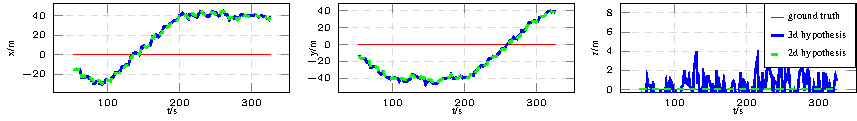
\includegraphics[width=1.0\textwidth]{./fig/plots/example_plot/hypotheses.pdf}
  \caption{Example of a 2D plot using \emph{PGFPlots}.}
  \label{fig:pgfplots}
\end{figure}

\section{3D Plots with Sketch}

\emph{Sketch} is a tool for defining a 3D scene using simple descriptive language.
The 3D scene is then converted to \emph{Tikz}, which is later compiled to pdf.
The benefits of using \emph{Sketch} are similar to using \emph{Tikz}: LaTeX fonts, versioning using git, and cleanness of the result.
See the example image in \reffig{fig:coordinate_systems}.
\begin{itemize}
  \item Documentation and manual: \url{http://www.frontiernet.net/~eugene.ressler/}
  \item Cross-compilation from \emph{Sketch} to \emph{pdf} using the \texttt{fig/sketch/compile\_sketch.sh} script.
\end{itemize}

\begin{figure}[!h]
  \centering
  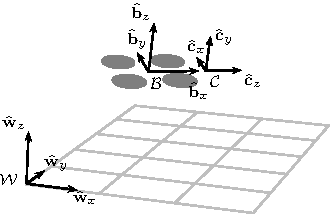
\includegraphics[width=0.4\textwidth]{./fig/sketch/coordinate_frames.pdf}
  \caption{Depiction of the used coordinate systems. The image was drawn using \emph{Sketch}.}
  \label{fig:coordinate_systems}
\end{figure}

\section{Image collages with Subfig}

We recommend using the \emph{subfig} packages, which provides the \emph{subfloat} command.
It is more versatile than the simpler \emph{subcaption} package.
Check the \reffig{fig:uavs} for example.

\begin{figure}[!h]
  \centering
  \subfloat[A UAV, the T650 model.] {
    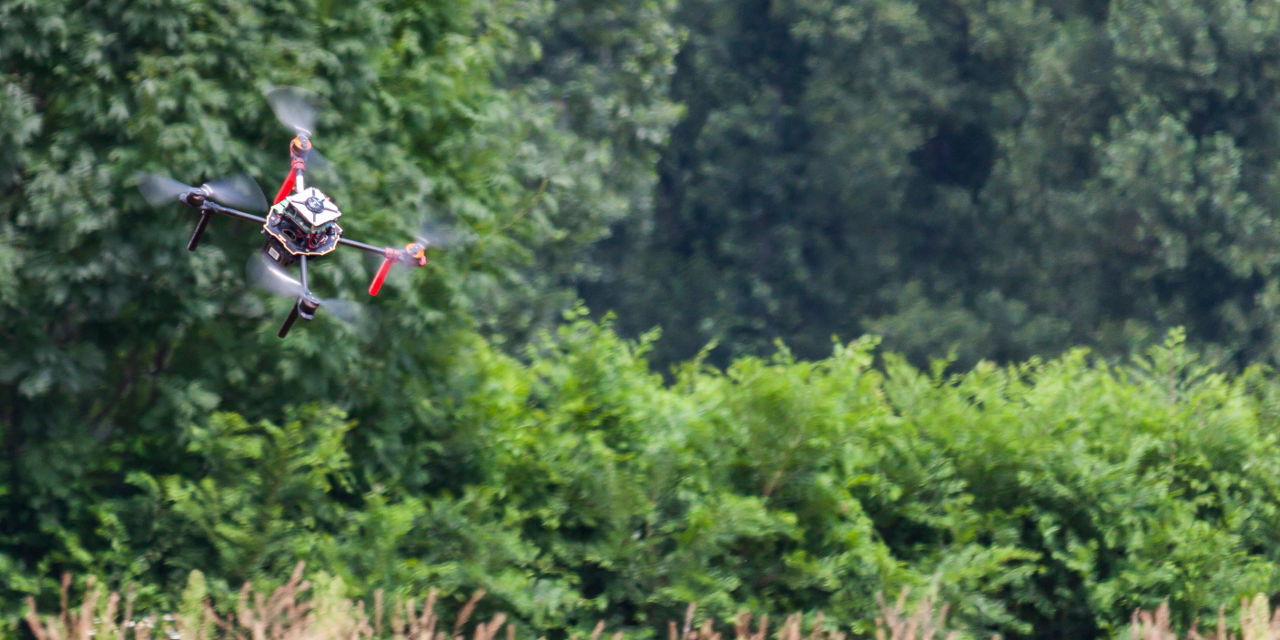
\includegraphics[width=0.48\textwidth]{./fig/photos/uav1.jpg}
    \label{fig:uavs_1}
  }
  \subfloat[Another UAV, again, T650 model.] {
    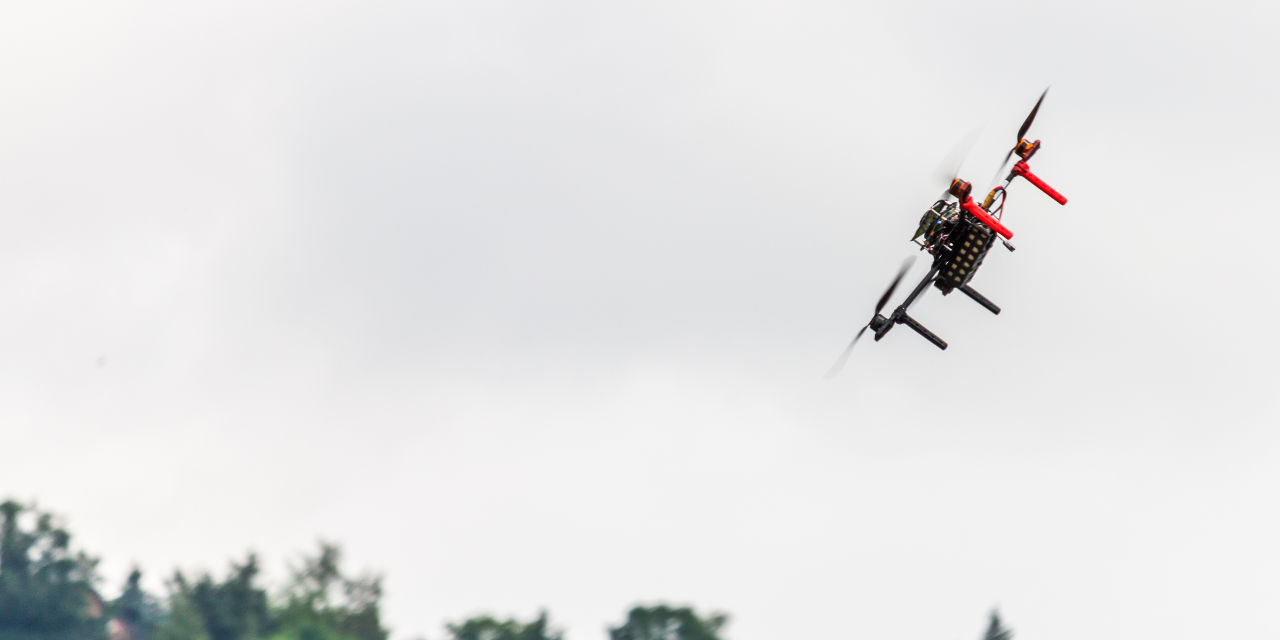
\includegraphics[width=0.48\textwidth]{./fig/photos/uav2.jpg}
    \label{fig:uavs_2}
  }
  \caption{The caption should mention both, the \reffig{fig:uavs_1} and the \reffig{fig:uavs_2}. You can just refer to them as (a) and (b), but beware, you need to keep it correct as you edit.}
  \label{fig:uavs}
\end{figure}

\section{Citations with Biblatex}

\emph{Biblatex} is probably the most powerful citation package for LaTeX.
It consumes the standard \texttt{.bib} file. However, it can sort and filter the citations using the \texttt{keywords} tag.
Citing references is done using the \texttt{cite} command, e.g., \cite{baca2021mrs}.
You can also define some nice citation boxes, such as this one:
\fullciteinbox{baca2021mrs}{}

\section{Image overlays with Tikz}

\emph{Tikz} is very useful to create custom image overlays.
The overlay can be set such that the image is spanned by Cartesian coordinates $\left(x, y\right) \in \left[0, 1\right]^2$
Example can be seen in \reffig{fig:tikz_overlay}.

\begin{figure}[!h]

  \centering

  \subfloat {\begin{tikzpicture}
    \node[anchor=south west,inner sep=0] (a) at (0,0) { 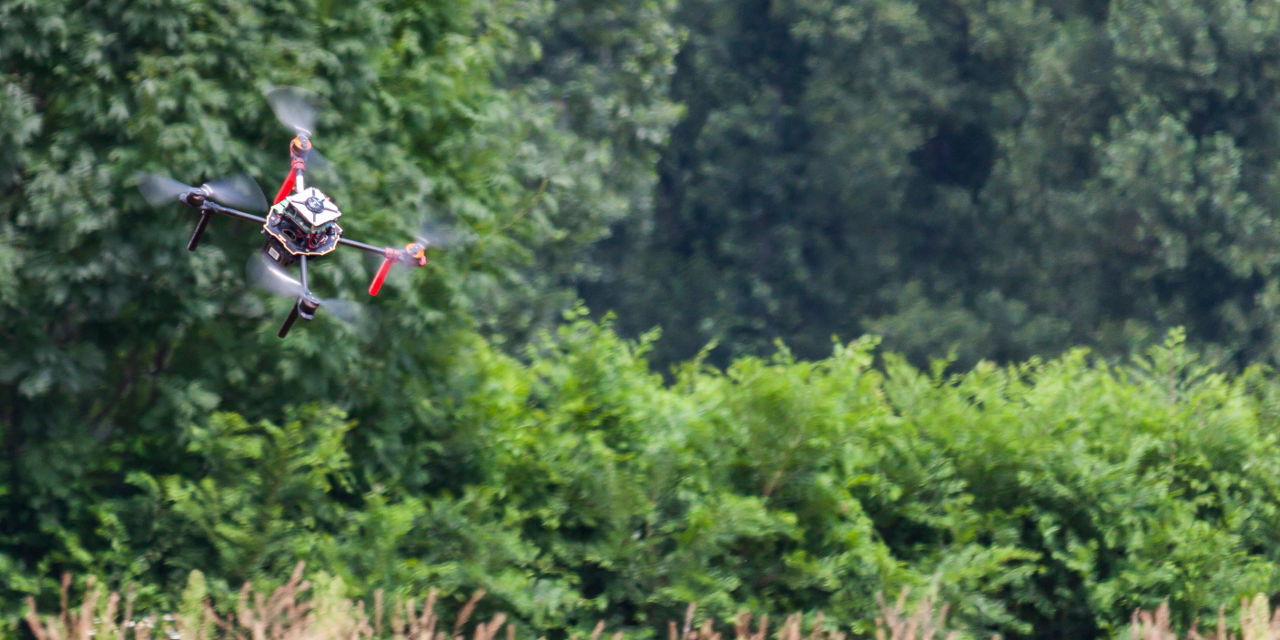
\includegraphics[width=0.45\textwidth]{./fig/photos/uav1.jpg}};
    \begin{scope}[x={(a.south east)},y={(a.north west)}]

      %%{ grid for placing the elements

      % % useful grid to help you find coordinates for plotting the overlay
      % \draw[black, xstep=.1, ystep=.1] (0,0) grid (1,1);
      % \foreach \i in {0,0.1,0.2,0.3,0.4,0.5,0.6,0.7,0.8,0.9,1} {
      %   \node[align=center] at (\i, -0.05) {\i};
      %   \node[align=center] at (\i, 1.05) {\i};
      %   \node[align=center] at (-0.05, \i) {\i};
      %   \node[align=center] at (1.05, \i) {\i};
      % }

      %%}

      % plot some stuff over the image

      % plot white background behind the letter (a)
      \fill[white] (0.001, 0.001) rectangle (0.10,0.14);

      % plot black border
      \fill[draw=black, draw opacity=0.5, fill opacity=0] (0,0) rectangle (1, 1);

      % write the letter (a) in the bottom-left corner
      \draw (0.05,0.06) node [text=black] {\small (a)};

      % plot black border
      \draw[->, white, thick] (0.50, 0.80) -- (0.30, 0.67);
      \draw (0.50,0.86) node [text=white] {\small \textbf{UAV}};
    \end{scope}
  \end{tikzpicture}}
\hfill%
\subfloat {\begin{tikzpicture}
    \node[anchor=south west,inner sep=0] (a) at (0,0) { 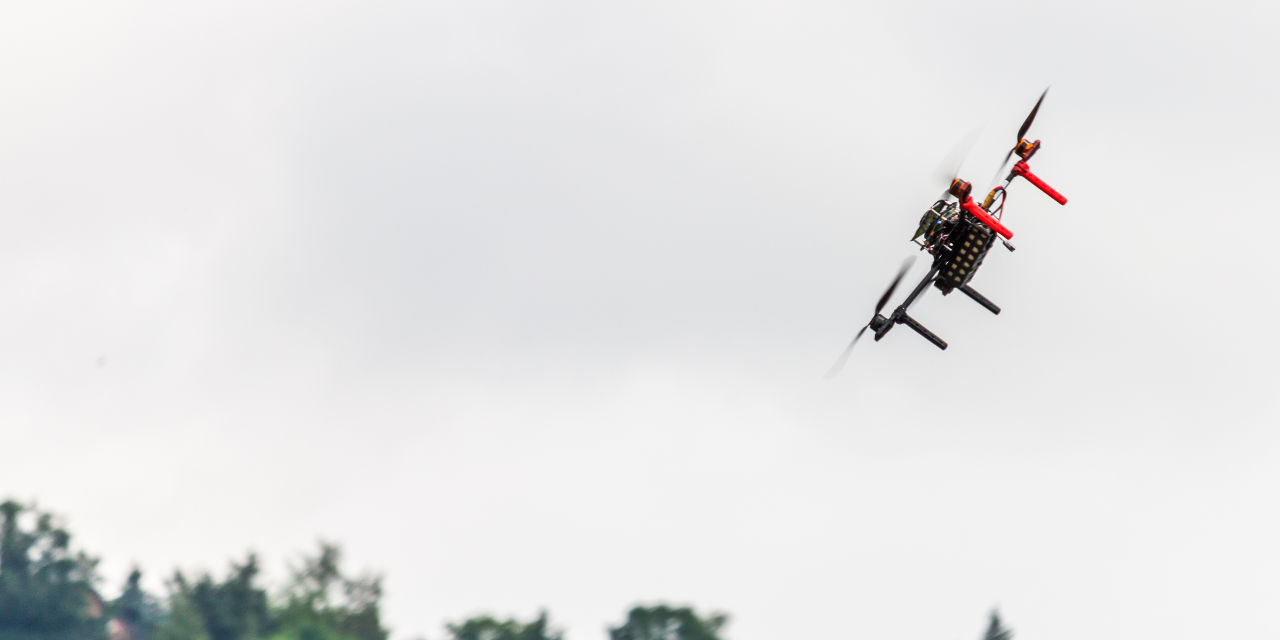
\includegraphics[width=0.45\textwidth]{./fig/photos/uav2.jpg}};
    \begin{scope}[x={(a.south east)},y={(a.north west)}]

      %%{ grid for placing the elements

      % useful grid to help you find coordinates for plotting the overlay
      \draw[black, xstep=.1, ystep=.1] (0,0) grid (1,1);
      \foreach \i in {0,0.1,0.2,0.3,0.4,0.5,0.6,0.7,0.8,0.9,1} {
        \node[align=center] at (\i, -0.05) {\i};
        \node[align=center] at (\i, 1.05) {\i};
        \node[align=center] at (-0.05, \i) {\i};
        \node[align=center] at (1.05, \i) {\i};
      }

      %%}

      % plot some stuff over the image

      % plot white background behind the letter (b)
      \fill[white] (0.001, 0.001) rectangle (0.10,0.14);

      % plot black border
      \fill[draw=black, draw opacity=0.5, fill opacity=0] (0,0) rectangle (1, 1);

      % write the letter (b) in the bottom-left corner
      \draw (0.05,0.06) node [text=black] {\small (b)};
    \end{scope}
  \end{tikzpicture}}


  \caption{Example of using Tikz for image overlays. (a) shows a final product, (b) shows a grid useful for nailing down the coordinates.}
  \label{fig:tikz_overlay}

\end{figure}


%% --------------------------------------------------------------
%% |                         Conclusion                         |
%% --------------------------------------------------------------

%!TEX root = ../main.tex

\chapter{Conclusion\label{chap:conclusion}}

Summarize the achieved results.


%% --------------------------------------------------------------
%% |                         Appendices                         |
%% --------------------------------------------------------------

\appendix
\renewcommand\chaptername{Appendix}

\chapter{References}

References to the author's work are listed first, followed by other references cited within this work.
The authored references contain his contribution and the number of citations based on Web~of~Science~(WoS), Scopus, and Google Scholar~(GS).
The citation counts were gathered on {\color{red} \texttt{insert date here}}.

\section{Thesis core publications}

\subsection*{Core articles in peer-reviewed journals}

\printbibliography[keyword={mine},keyword={phd_related},keyword={journal},keyword={core},notkeyword={submitted},heading=none,title={}]

\section{Thesis-related author's publications}

\subsection*{Thesis-related conference articles}

\printbibliography[keyword={mine},keyword={phd_related},keyword={conference},notkeyword={core},notkeyword={submitted},heading=none,title={}]

\section{Cited references}

\printbibliography[notkeyword=mine,heading=none,title={}]

% \appendix
\renewcommand{\thechapter}{B}
\renewcommand\chaptername{Appendix B}

\chapter{Appendix B}

\end{document}
